\documentclass[a4paper, 10pt]{article}

\usepackage[utf8]{inputenc}
\usepackage[spanish]{babel}
\usepackage{graphicx}
\usepackage{geometry}
\usepackage{listings}
\usepackage{amsmath}
\usepackage{amsfonts}
\usepackage{amssymb}
\usepackage{caratula}
\usepackage[section]{placeins}
\usepackage{titlesec}

\newcommand{\Z}{\mathbb{Z}}
\def\code#1{\texttt{#1}}
\newcommand\tab[1][0.5cm]{\hspace*{#1}}

\geometry{a4paper, margin=0.7in}

\begin{document}
    %Caratula
    \pagenumbering{gobble}
    \newpage

    \begin{center}
        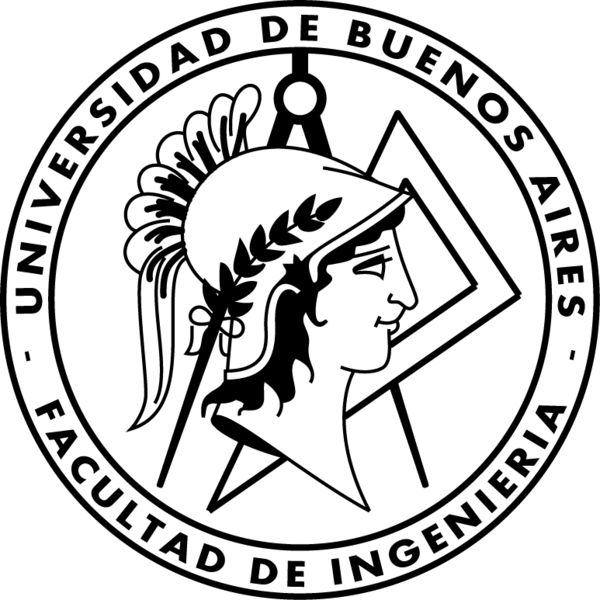
\includegraphics[width=7.5cm, height=7.5cm]{images/logo}
    \end{center}

    \materia{Organización de Datos}
    \submateria{Segundo Cuatrimestre 2017}
    \titulo{Trabajo Práctico 1}

    \integrante{Rodrigo De Rosa}{97799}{rodrigoderosa@outlook.com}
    \integrante{Marcos Schapira}{97934}{schapiramarcos@gmail.com}
    \integrante{Facundo Guerrero}{97981}{facundoiguerrero@gmail.com}
    \maketitle
    %Fin caratula
    %Table of contents
    \newpage
    \pagenumbering{roman}
    \tableofcontents
    %Fin table of contents
    %Informe
    \newpage
	\pagenumbering{arabic}
	\part{Análisis del tipo de las propiedades}
		En esta parte, se analizará como las distintas características de las propiedades son afectadas por el tipo de propiedad.
		Esto es, si son negocios, casas, PHs o departamentos.
		\section{Tipos de propiedades y sus superficies}
			\subsection{¿Dónde están las propiedades más grandes según su tipo?}
				%Bottom 5				
				\subsubsection{Casas}
				\subsubsection{PHs}
				\subsubsection{Departamentos}
				\subsubsection{Locales}
			\subsection{¿Dónde están las propiedades más chicas según su tipo?}
				%Top 5				
				\subsubsection{Casas}
				\subsubsection{PHs}
				\subsubsection{Departamentos}
				\subsubsection{Locales}
		\section{Tipos de propiedades y sus precios}
			\subsection{¿Dónde están las propiedades más caras según su tipo?}
				%Top 5				
				\subsubsection{Casas}
				\subsubsection{PHs}
				\subsubsection{Departamentos}
				\subsubsection{Locales}
			\subsection{¿Dónde están las propiedades más baratas según su tipo?}
				%Bottom 5				
				\subsubsection{Casas}
				\subsubsection{PHs}
				\subsubsection{Departamentos}
				\subsubsection{Locales}
		\section{Tipos de propiedades y sus ubicaciones}
			\subsection{¿En qué lugar hay más propiedades de cada tipo?}
				%Top 5 (heat-map)
				\subsubsection{Casas}
				\subsubsection{PHs}
				\subsubsection{Departamentos}
				\subsubsection{Locales}
		\section{Variación del precio total a través de los años}
			\subsection{Casas}
			\subsection{PHs}
			\subsection{Departamentos}
			\subsection{Locales}
		\section{Variación del precio por $m^2$ a través de los años}
			\subsection{¿Cuál fue el tipo de propiedad más caro en cada año?}
				\subsubsection{2013}
				\subsubsection{2014}
				\subsubsection{2015}
				\subsubsection{2016}
				\subsubsection{2017}
			\subsection{Casas}
			\subsection{PHs}
			\subsection{Departamentos}
			\subsection{Locales}
			\subsection{Análisis conjunto}
		
\end{document}